
%------------------------------------------------------------------------
% Anhänge
\appendix
\chapter{Appendix}
\section{Quellcode}

\lstset{% general command to set parameter(s)
	basicstyle=\small\ttfamily,%\small, % print whole listing small
	keywordstyle=\color{THIblue}\bfseries,% underlined boldblack keywords
	numbers=left,
	numberstyle=\color{gray},
	numbersep=5pt,
	captionpos=t}

\lstset{language=C}

\lstinputlisting[caption=Blink\_2.ino,language=c]{documents/Blink_2.ino}

%setcounter{XX}{To}

\newpage
\section{Ergänzende Grafiken}

\begin{figure}[htbp]
\centering
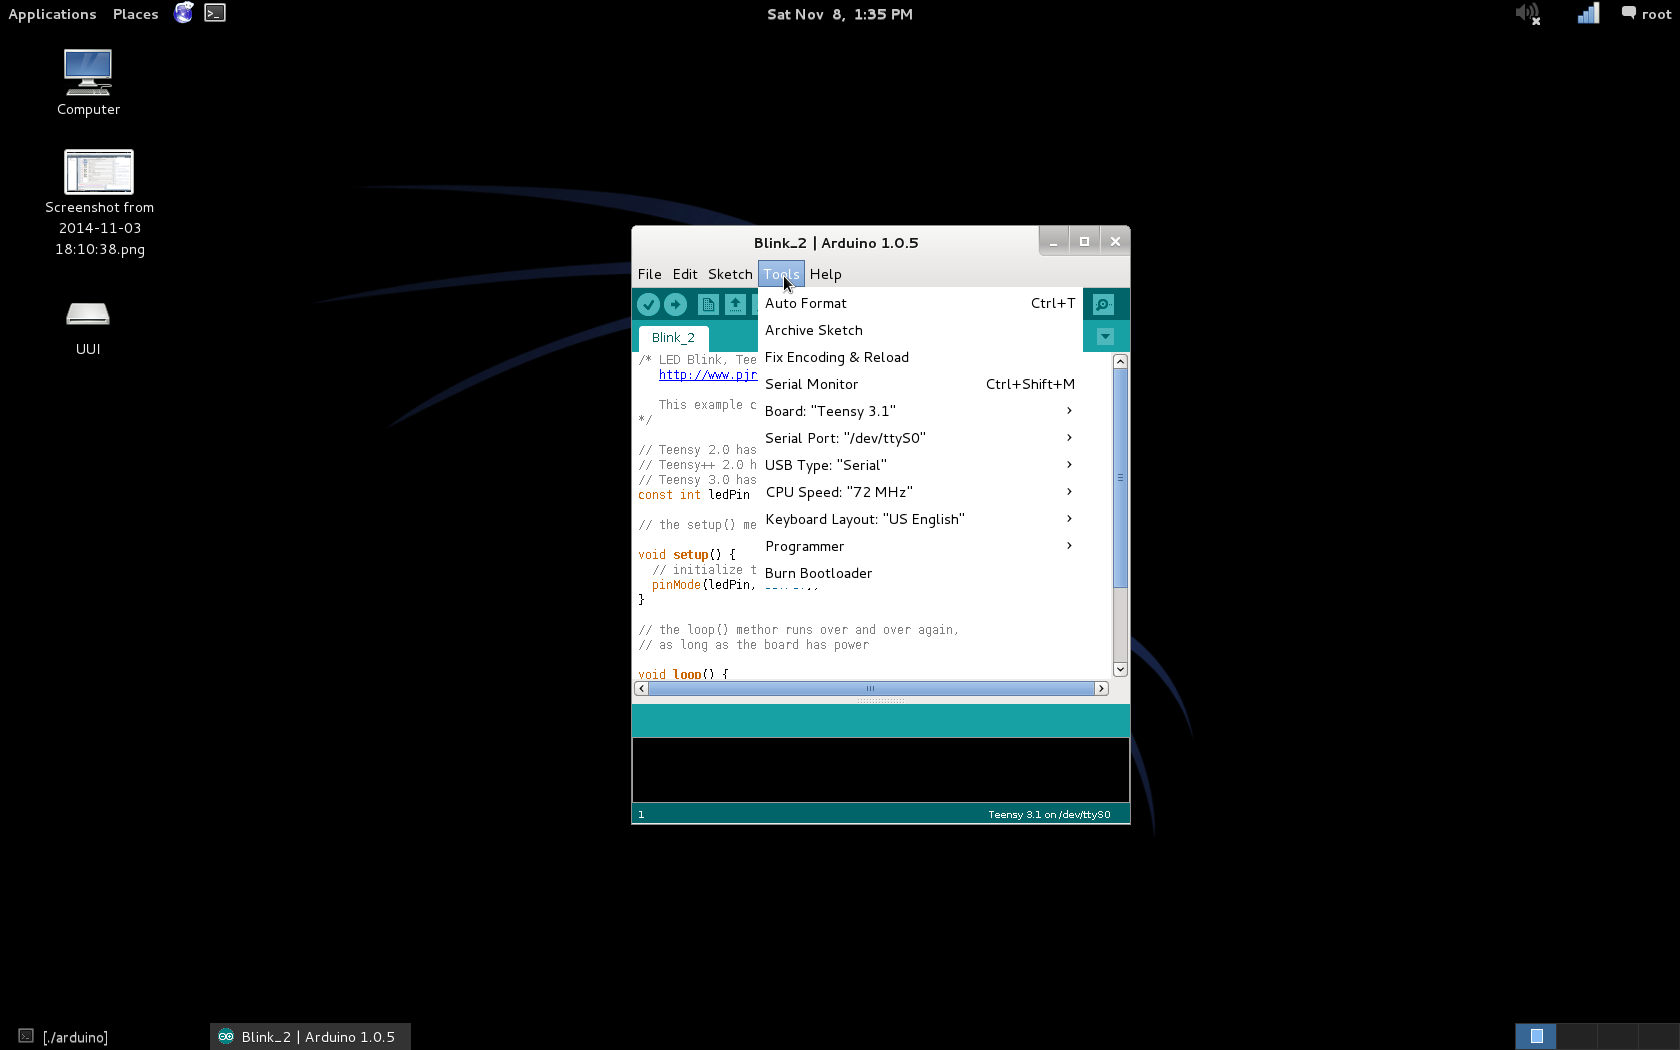
\includegraphics[width=\textwidth]{bilder/EinstellungenArduino2.png}
\caption{Einstellungen Arduino}
\label{fig:EinstellungenArduino}
\end{figure}

\section{Quellcode Grafiken}
\lstset{language=tikz}

\lstinputlisting[caption={Ablaufdiagramm \ref{fig:Ablauf}}]{chapter/ablaufGrafik}

\lstinputlisting[caption={USB Deskriptoren \ref{fig:usbDeskriptoren}}]{chapter/usbDeskriptoren}
